\documentclass[12pt]{article}%
    \usepackage[final]{pdfpages}
    \usepackage{listings} %For code in appendix
    \usepackage{hyperref}
    \lstset
    { %Formatting for code in appendix
        language=c++,
        basicstyle=\footnotesize,
        numbers=left,
        stepnumber=1,
        showstringspaces=false,
        tabsize=1,
        breaklines=true,
        breakatwhitespace=false,
    }
    \title{Lab 2}
    \date {2nd week}
    \author{FIT Staff}
    \begin{document}
    \maketitle
    \section{topics}
    \begin{itemize}
        \item bit manipulation, or, xor, and, shift left, shift right
        \item if else operator
        \item loop operators: for, while, do while
    \end{itemize}
    
    \section{reading materials}
    in russian:
    \begin{itemize}
        \item \url{https://informatics.msk.ru/mod/book/view.php?id=547}
        \item \url{https://informatics.msk.ru/mod/book/view.php?id=550}
        \item \url{https://informatics.msk.ru/mod/book/view.php?id=557}
    \end{itemize}
    in english:
    \begin{itemize}
        \item \url{https://en.cppreference.com/w/cpp/language/if}
        \item \url{https://en.cppreference.com/w/cpp/language/for}
        \item \url{https://en.cppreference.com/w/cpp/language/while}
        \item \url{https://cprogramming.com/tutorial/bitwise_operators.html}
    \end{itemize}

    \section{problem set}
    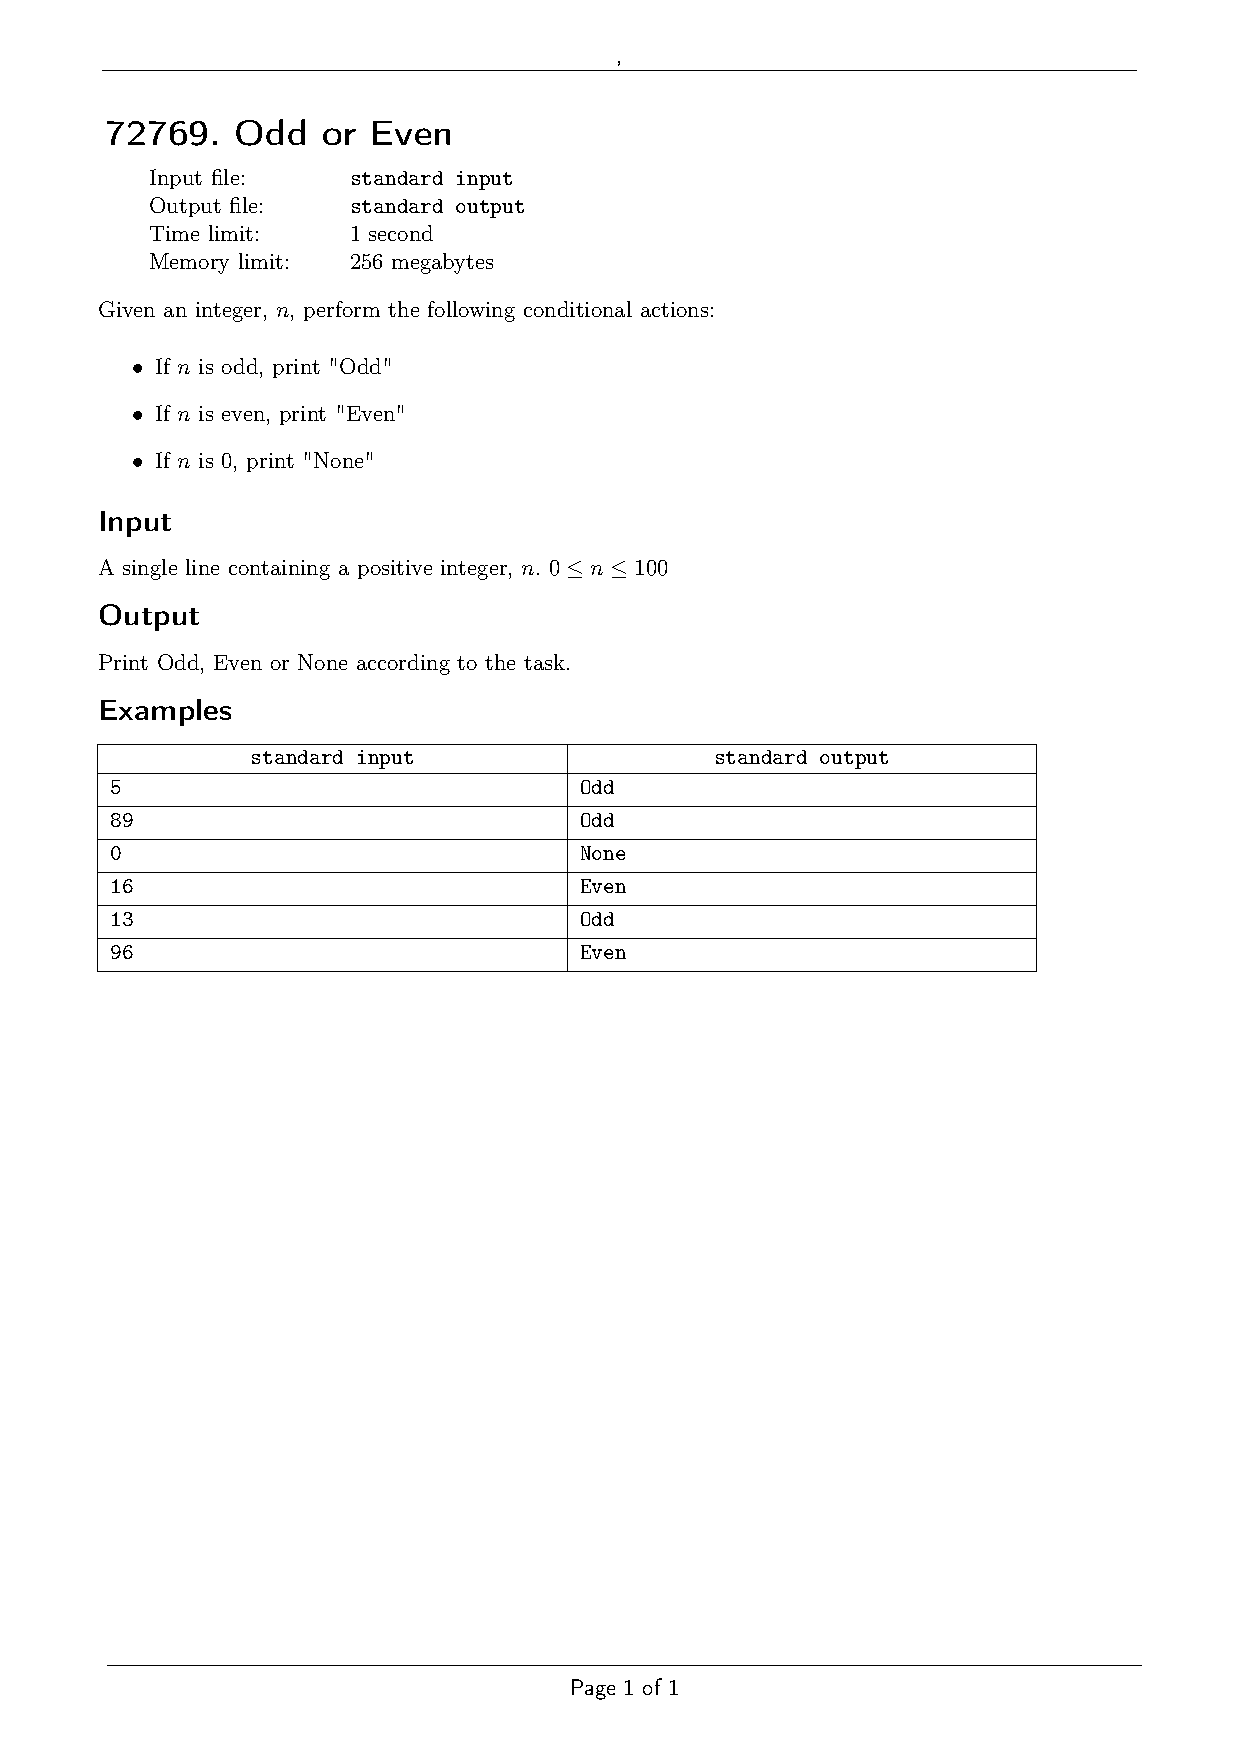
\includepdf[pages=-]{72769.pdf}
    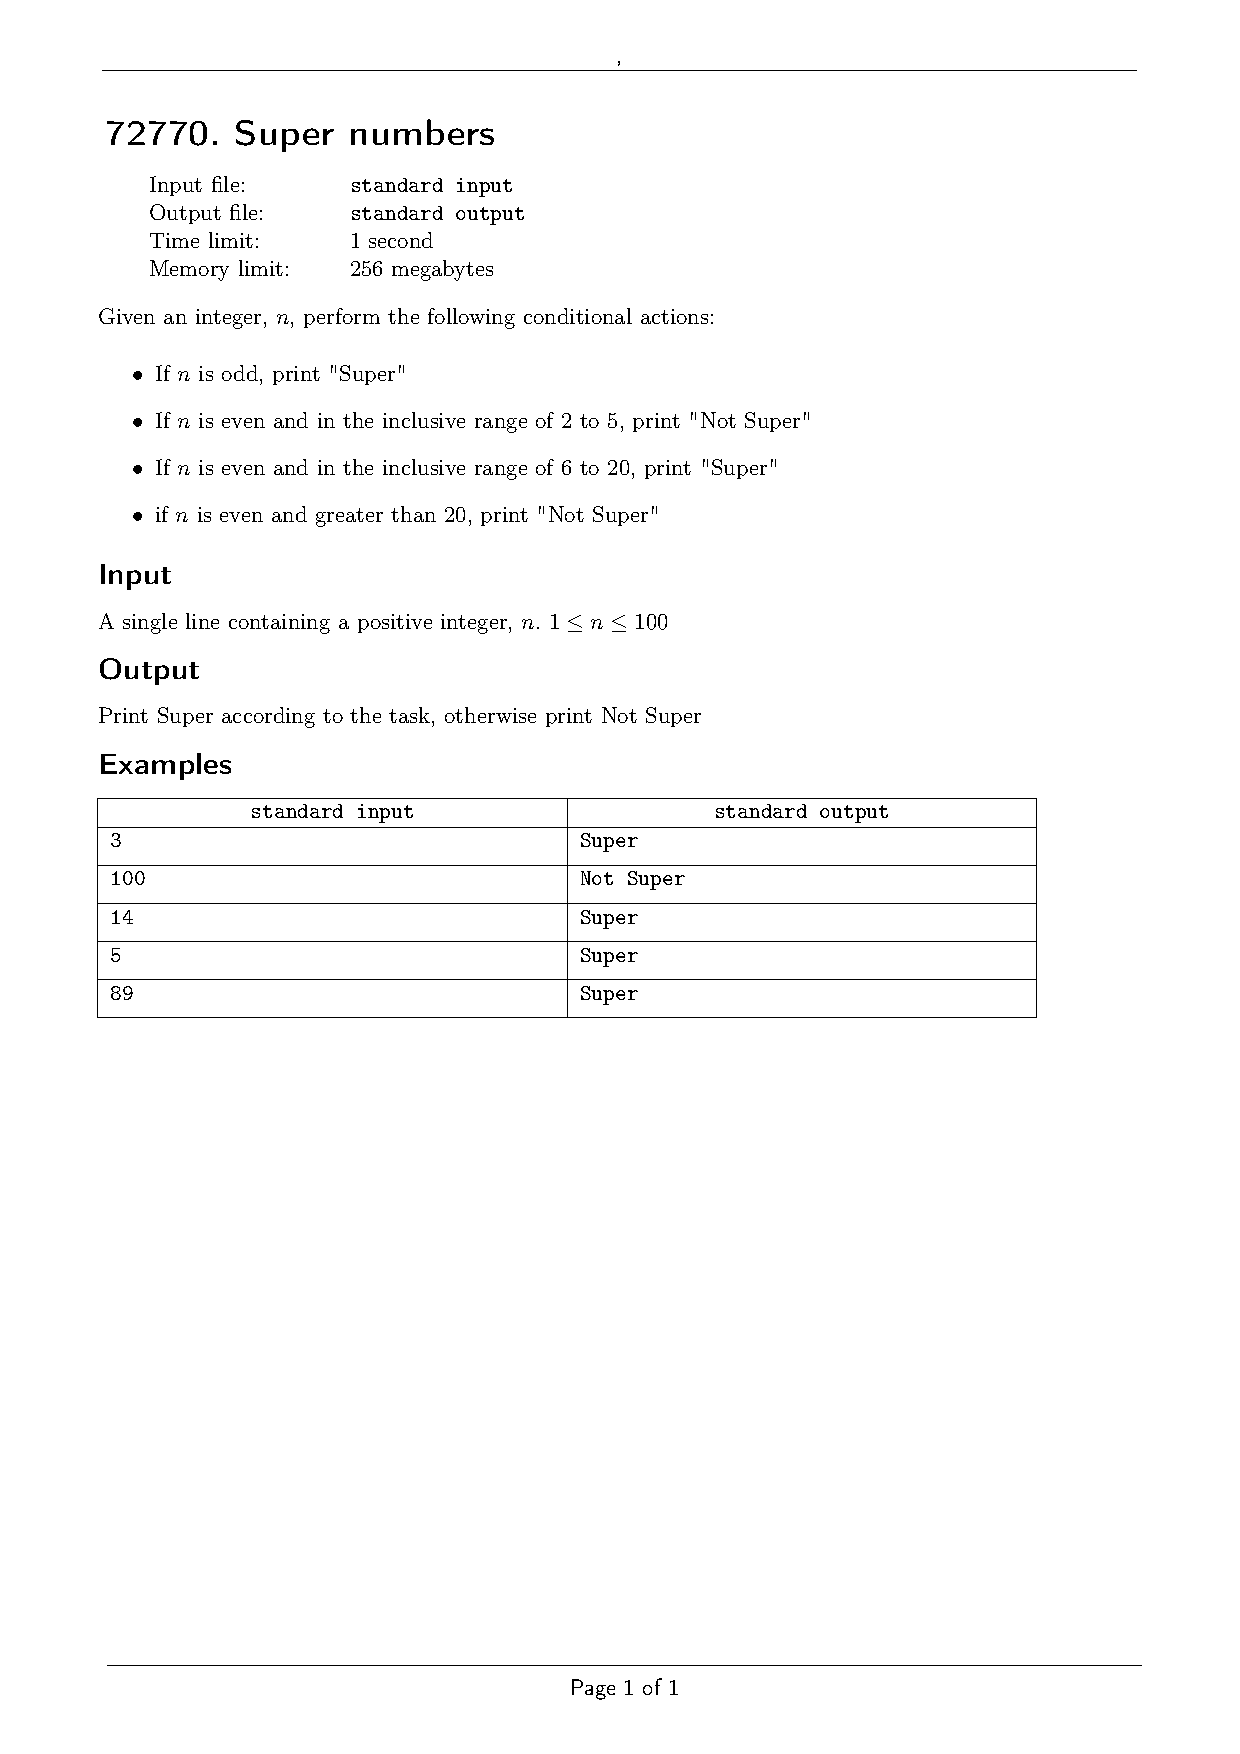
\includepdf[pages=-]{72770.pdf}
    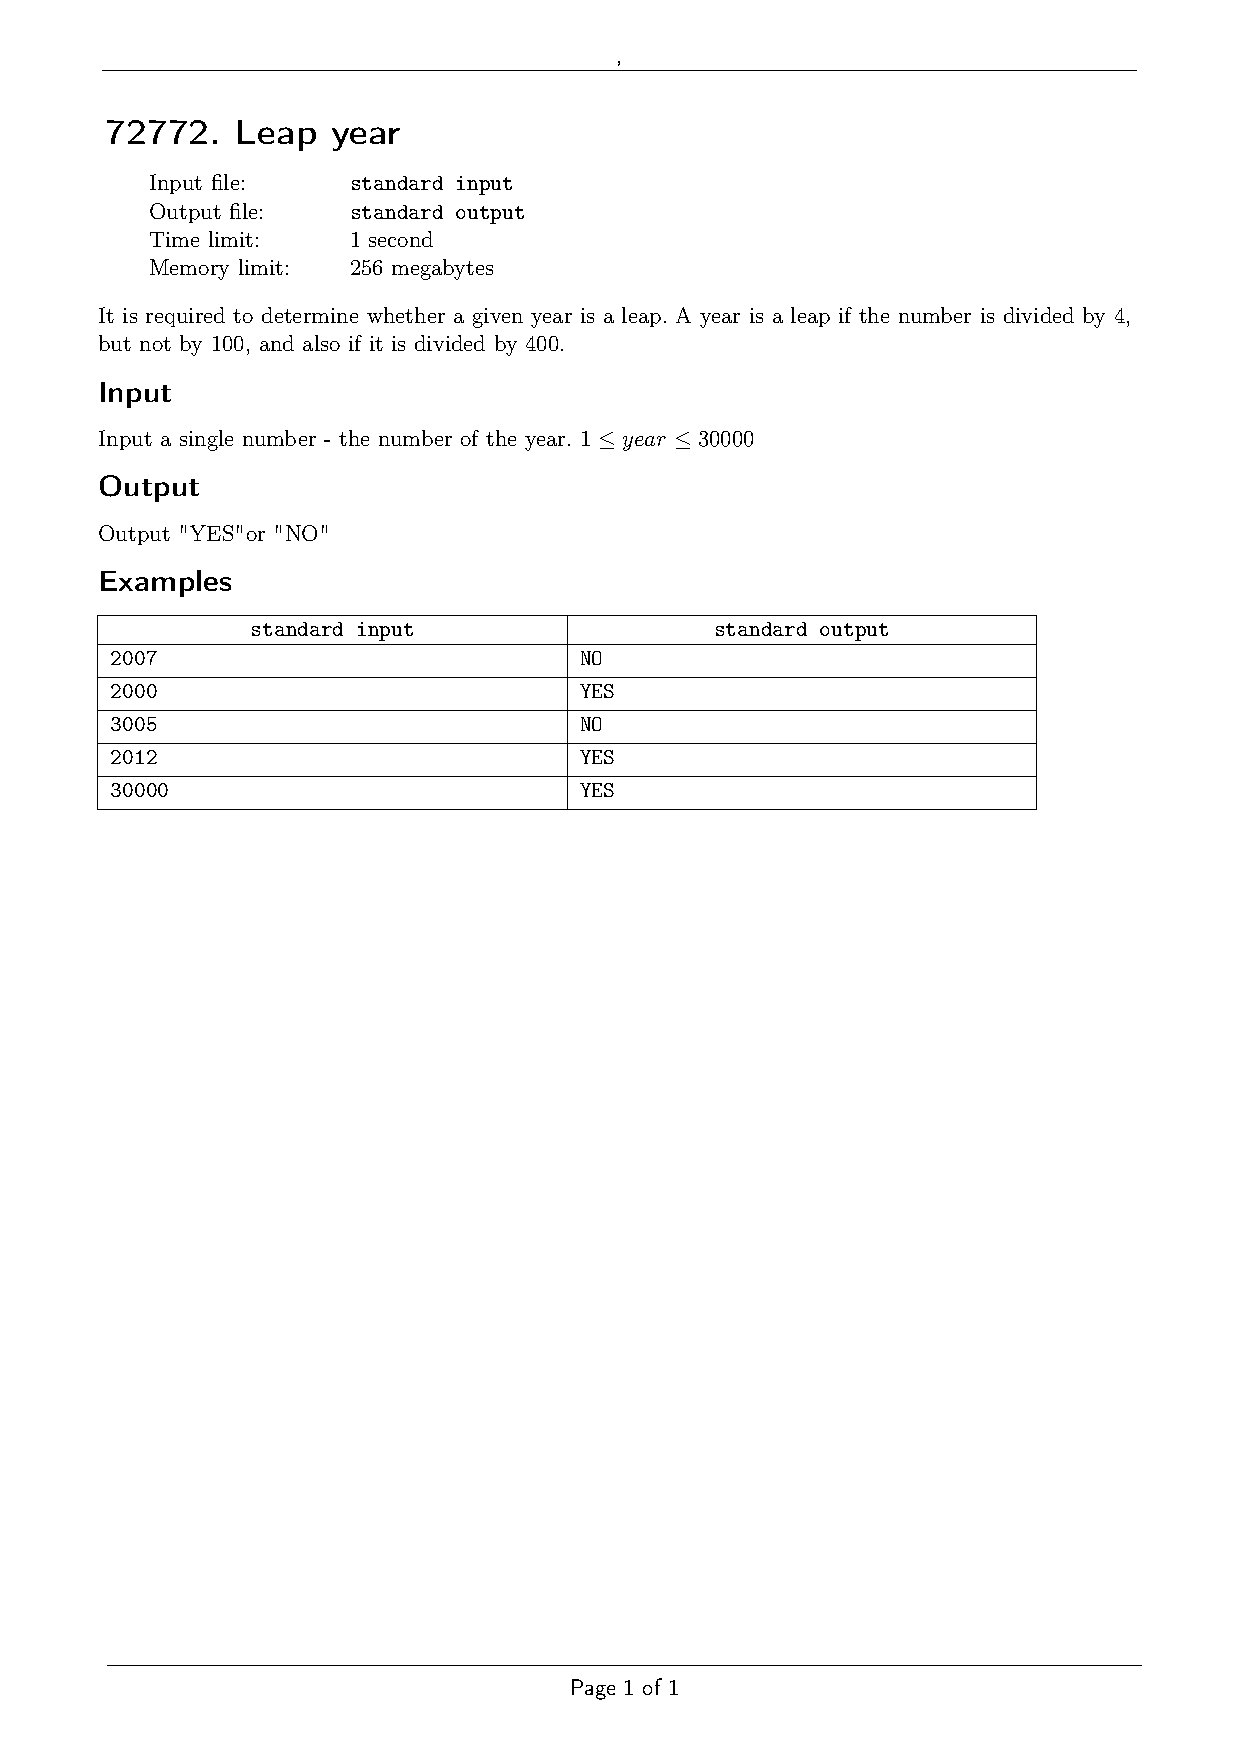
\includepdf[pages=-]{72772.pdf}
    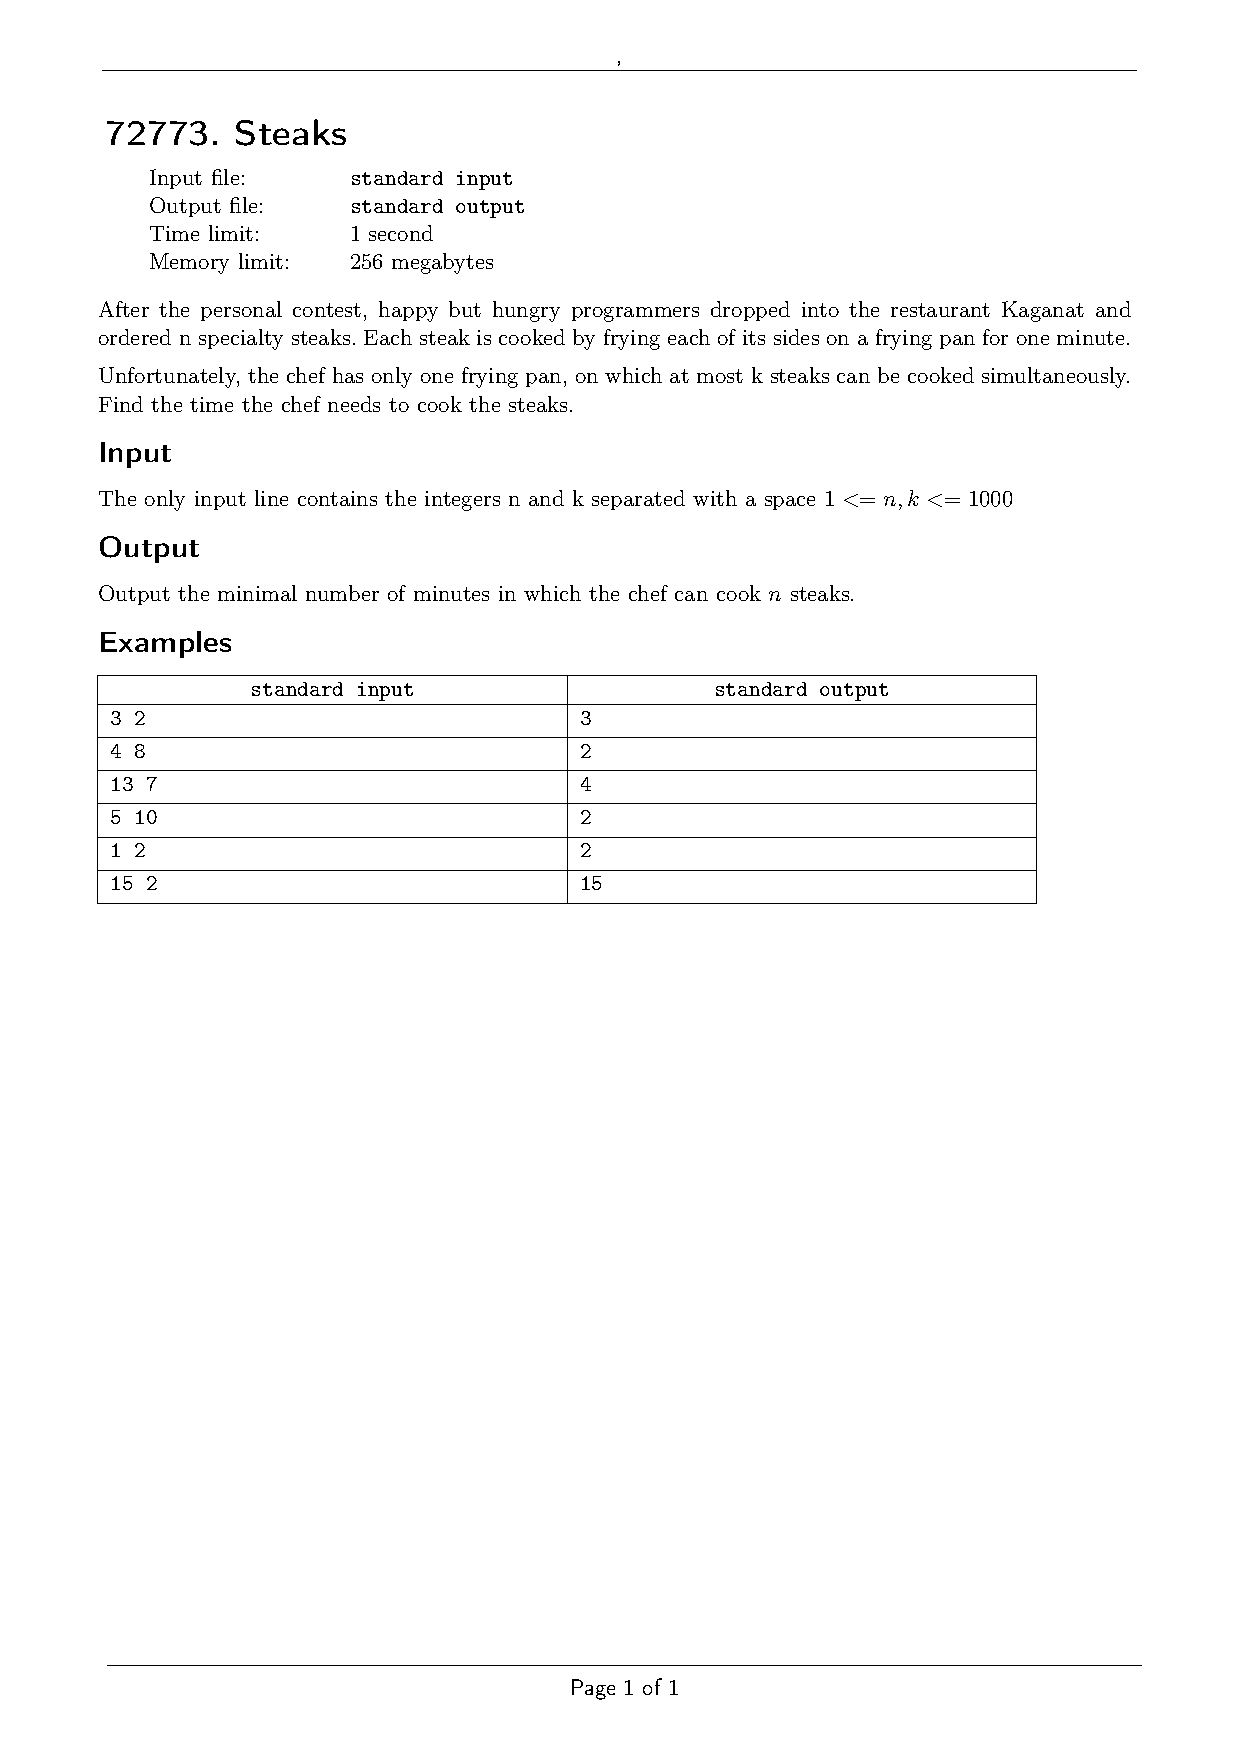
\includepdf[pages=-]{72773.pdf}
    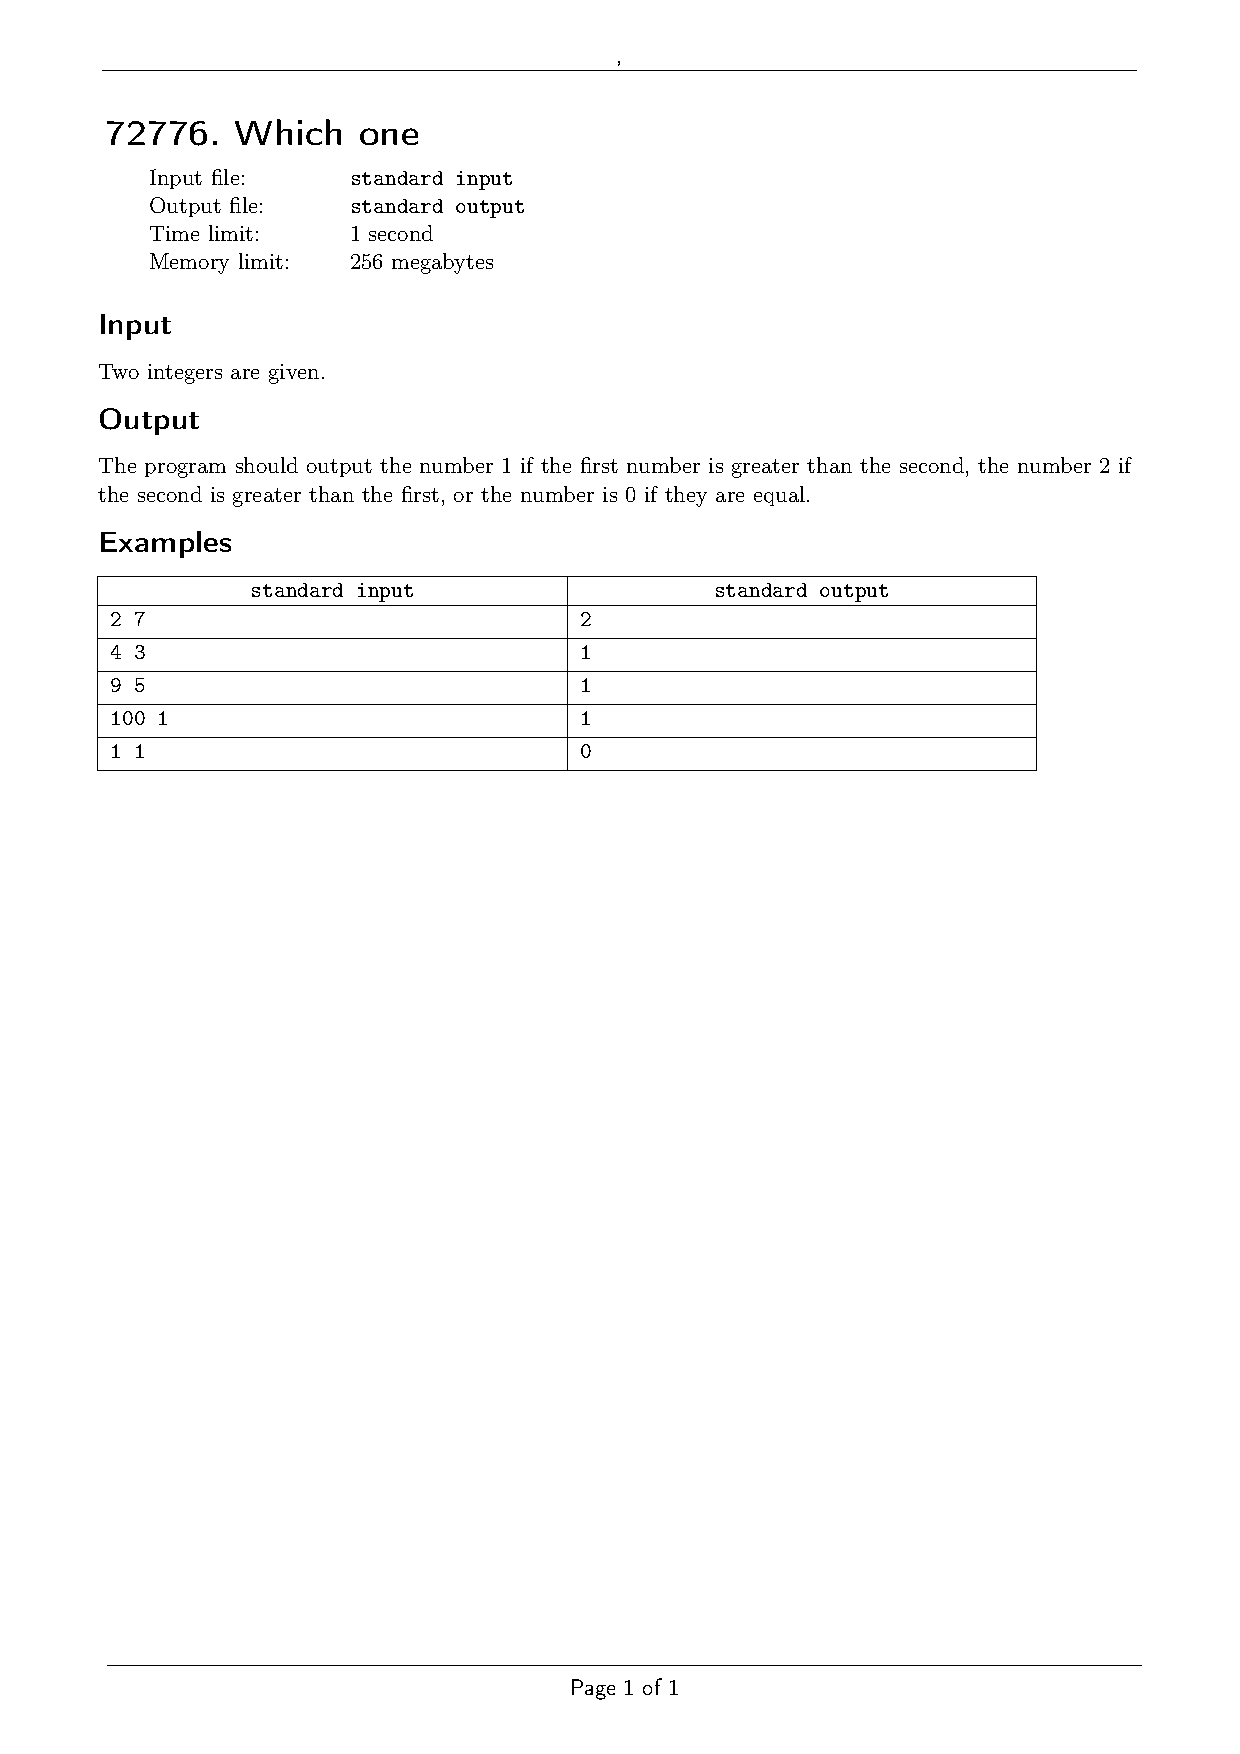
\includepdf[pages=-]{72776.pdf}
    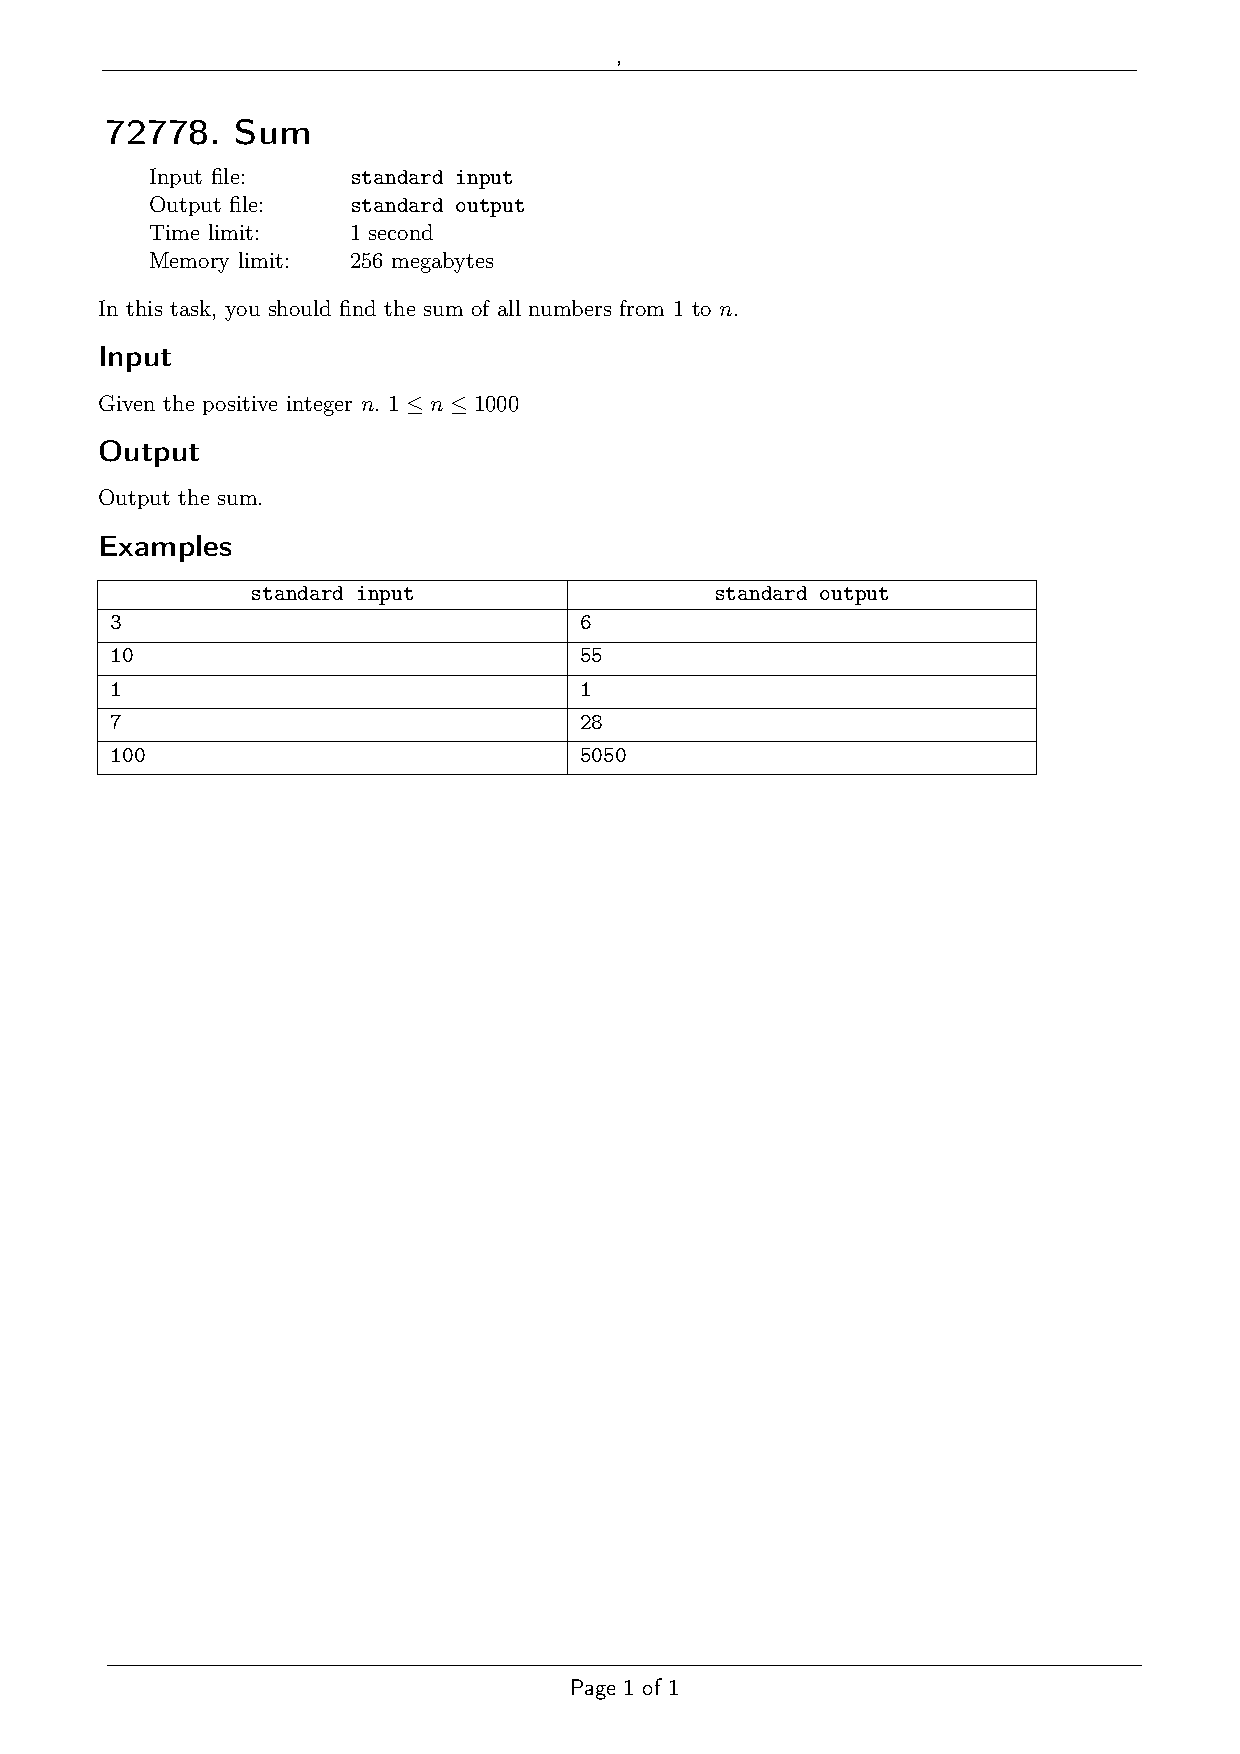
\includepdf[pages=-]{72778.pdf}
    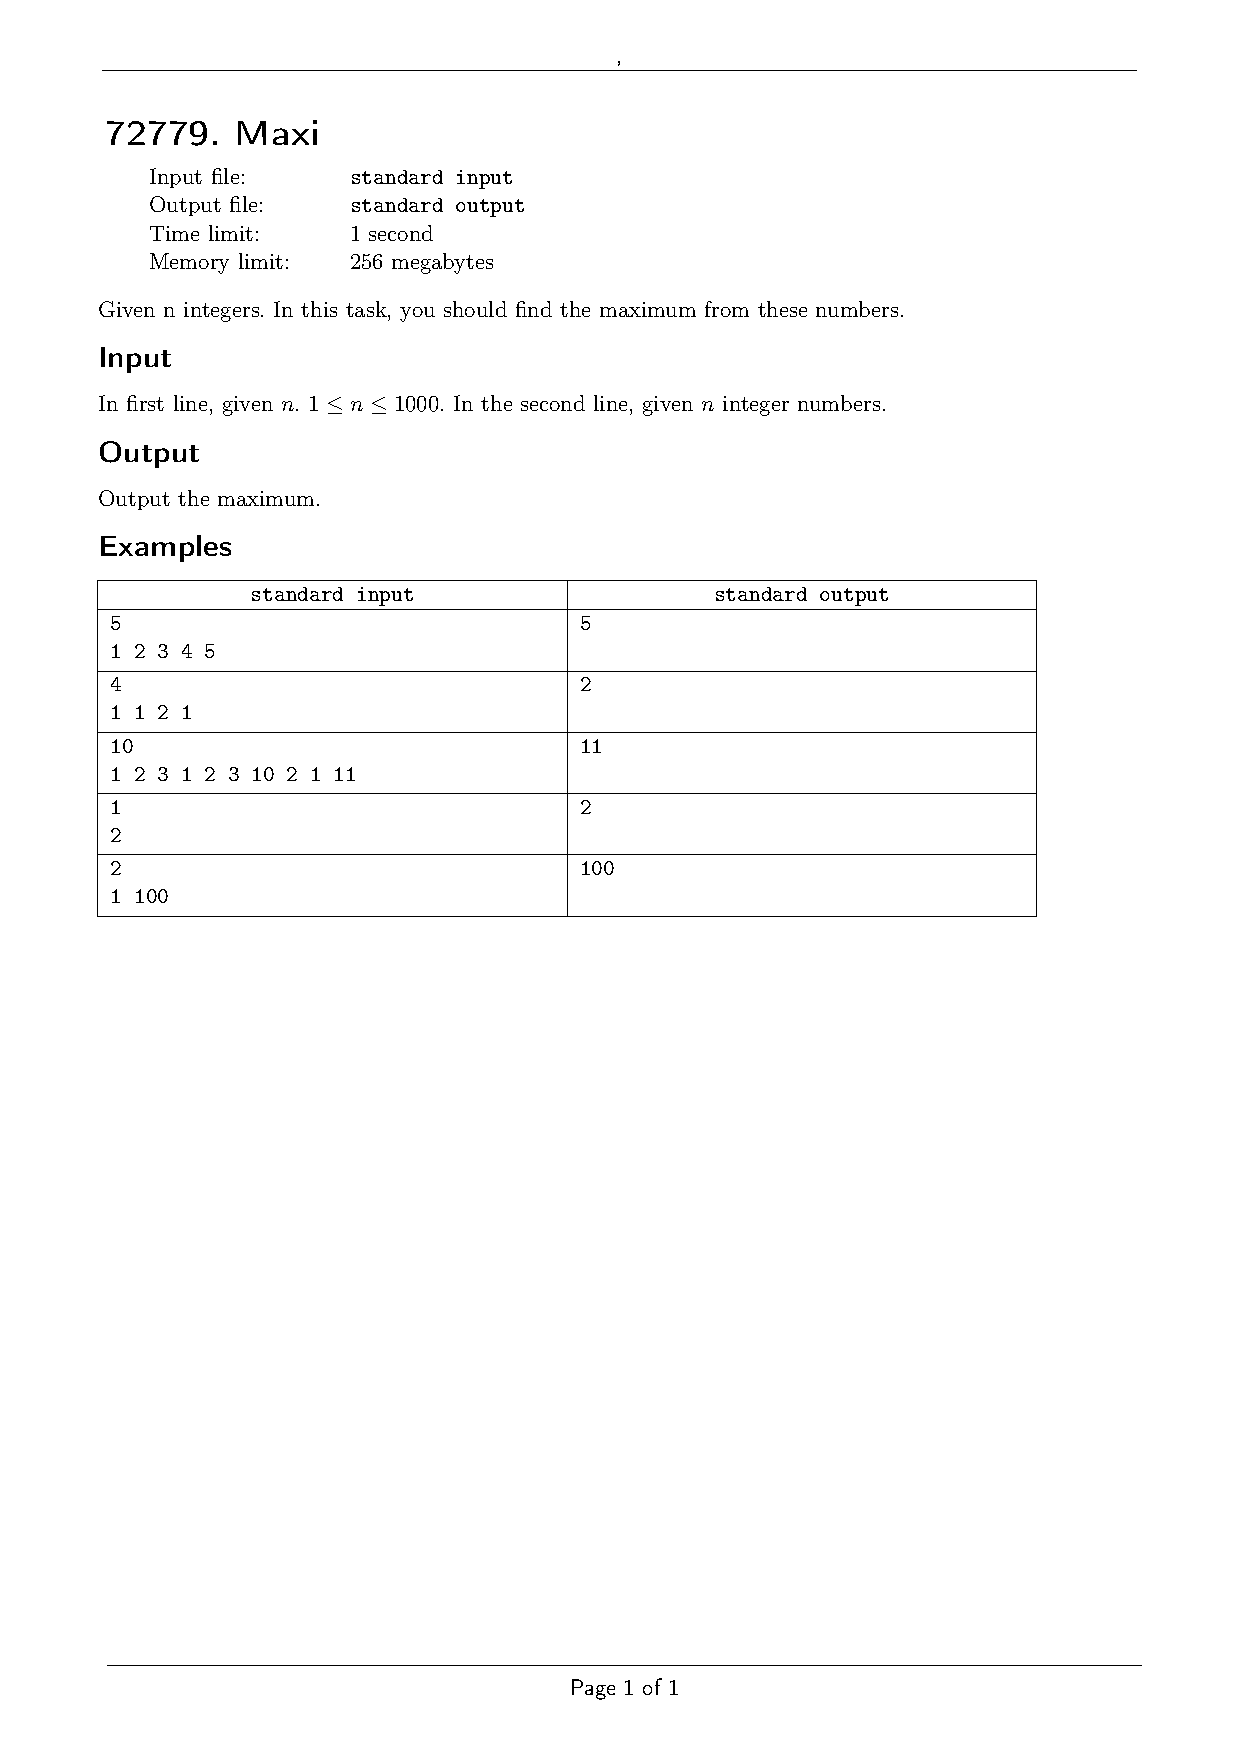
\includepdf[pages=-]{72779.pdf}
    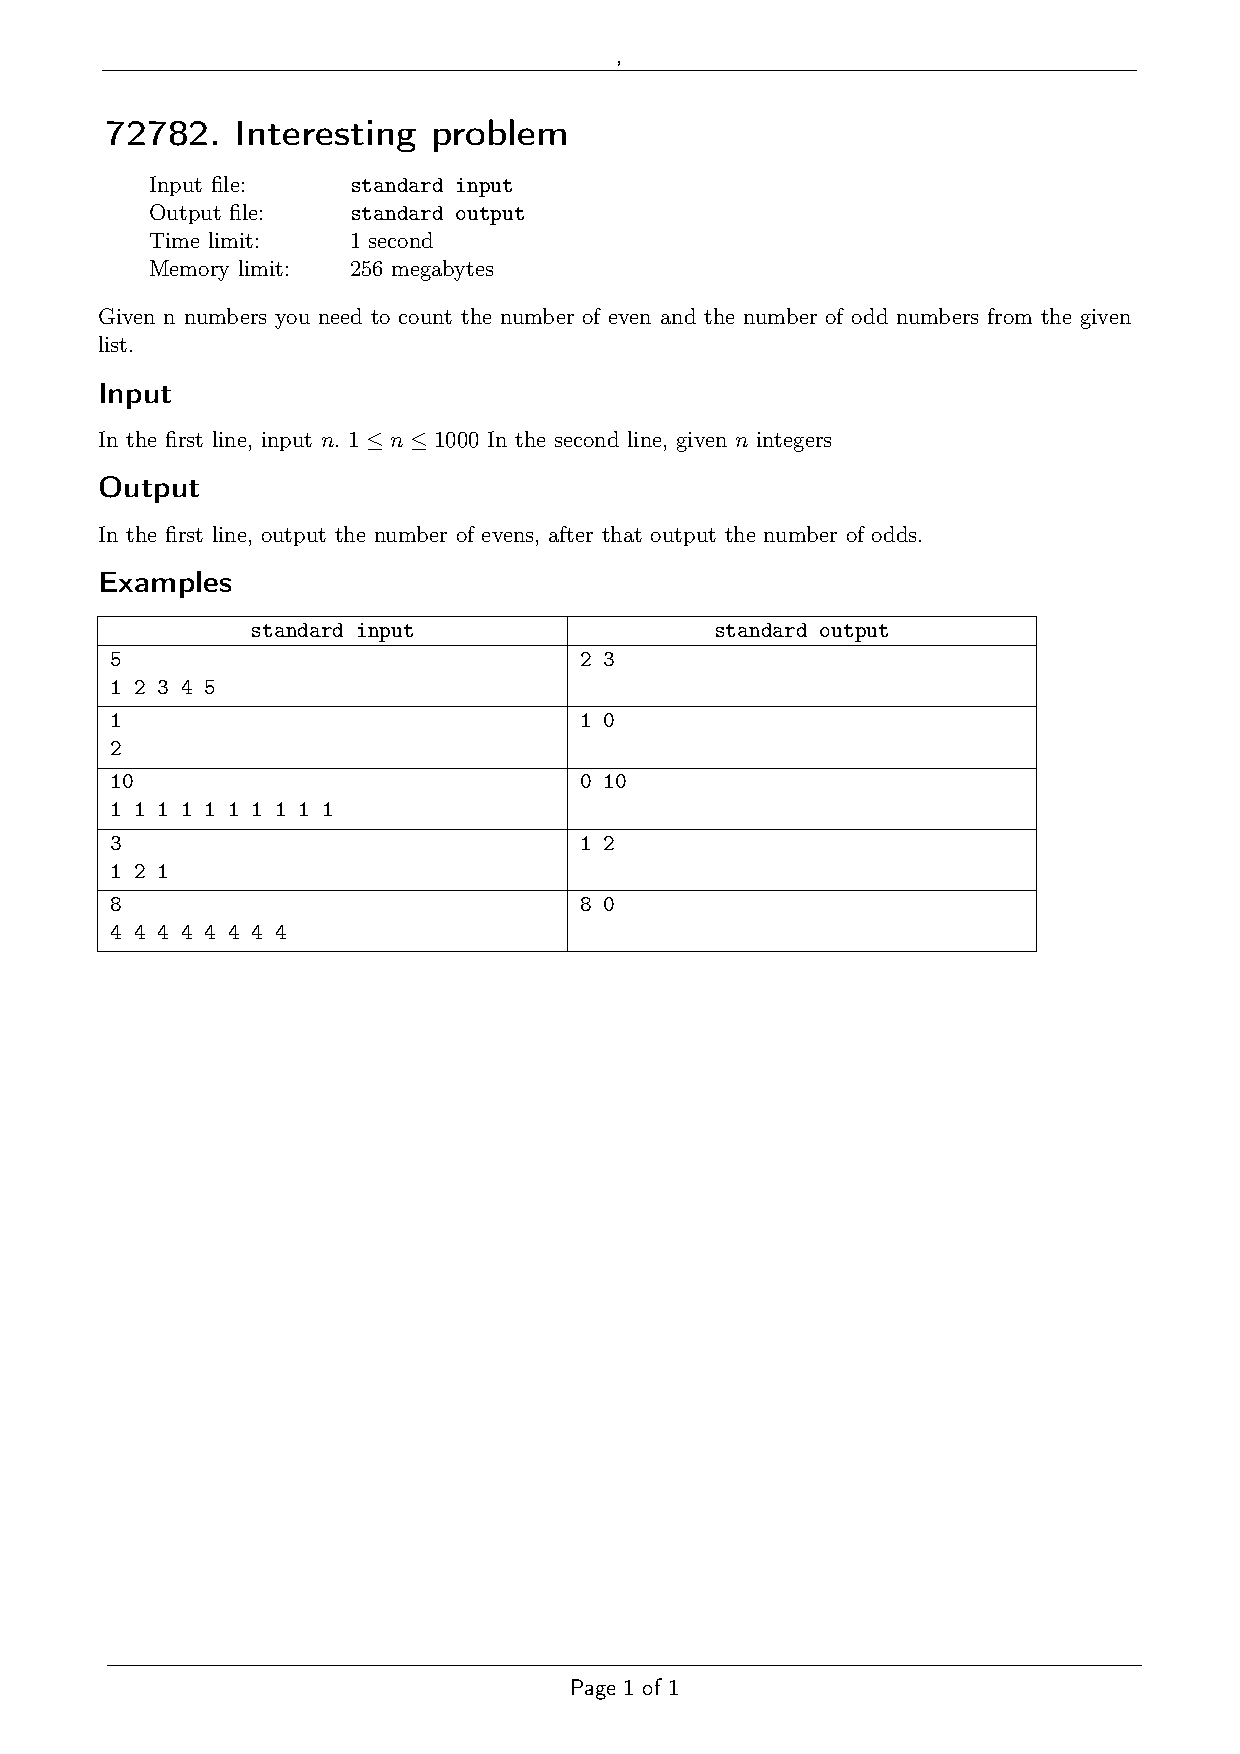
\includepdf[pages=-]{72782.pdf}
    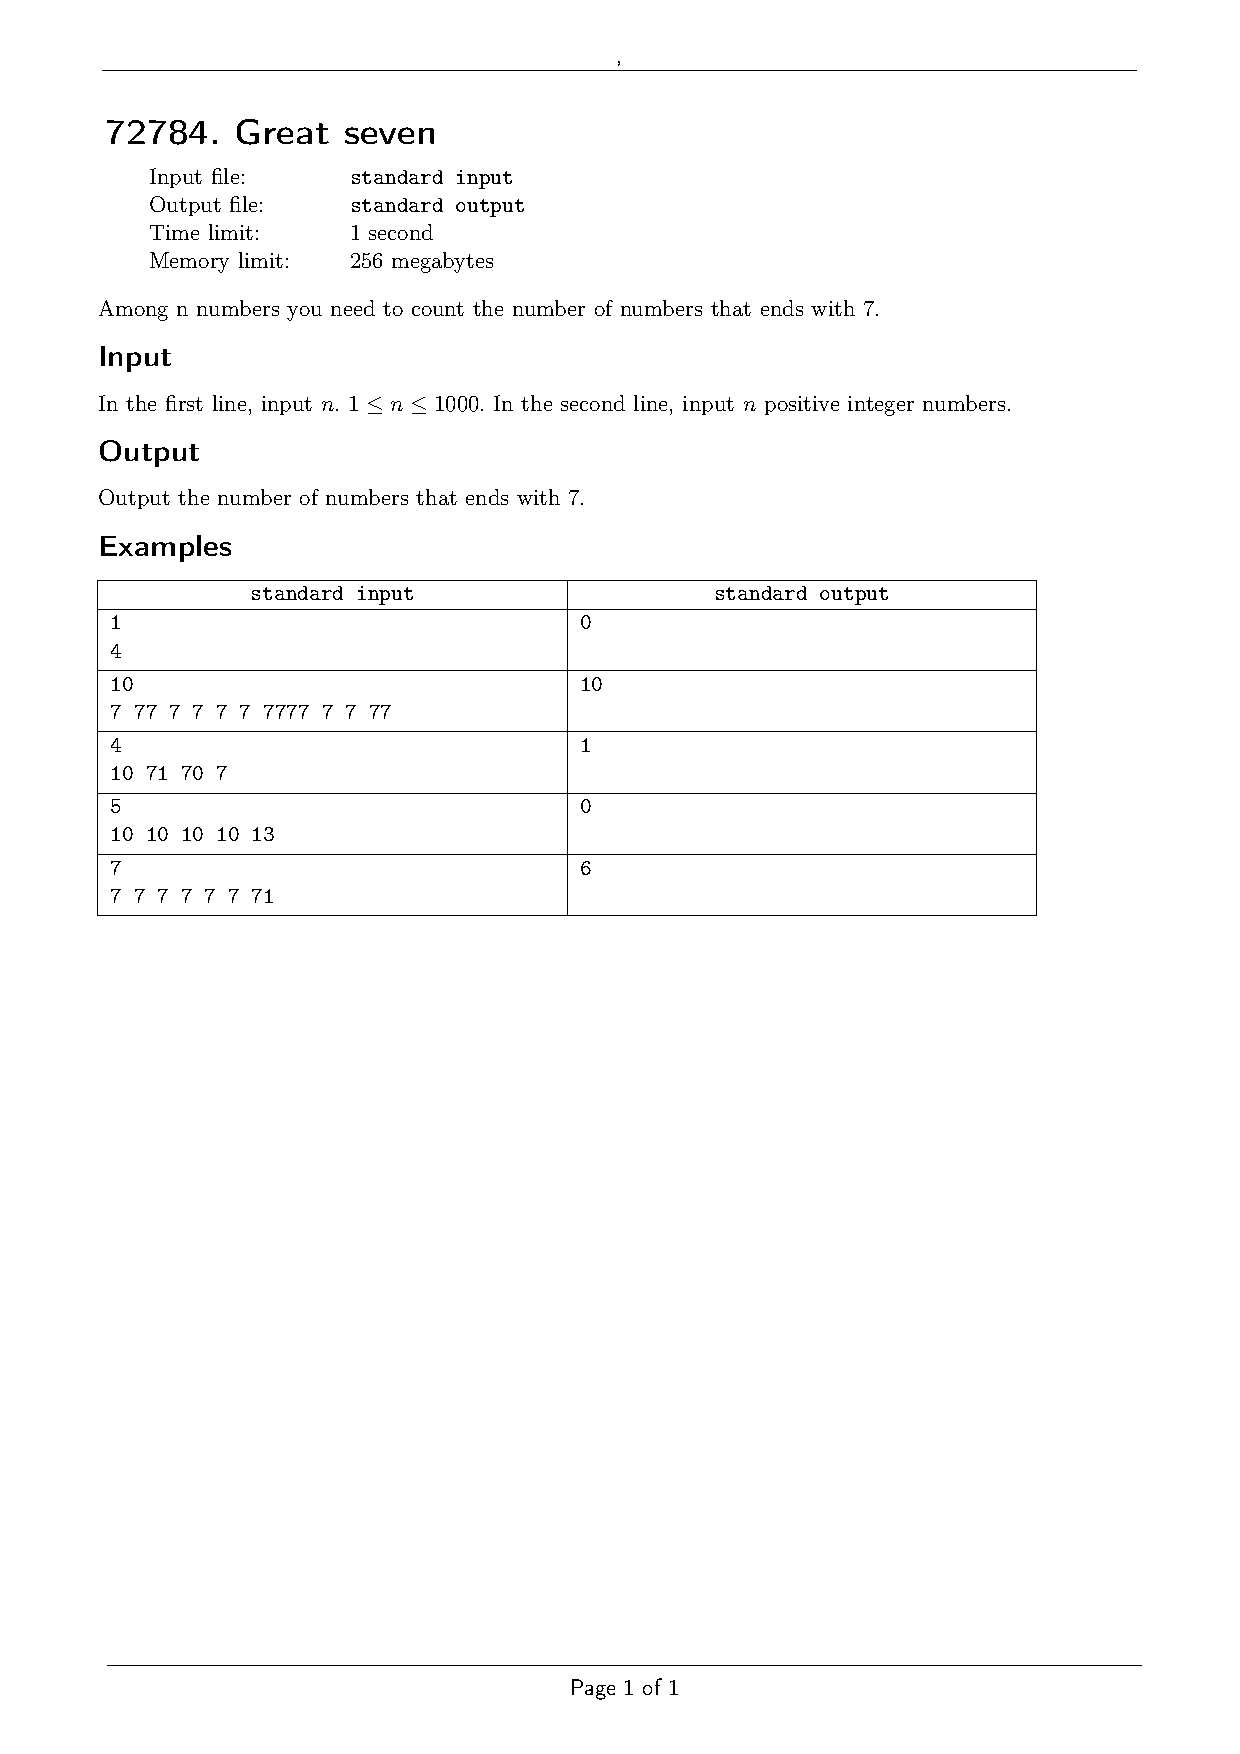
\includepdf[pages=-]{72784.pdf}
    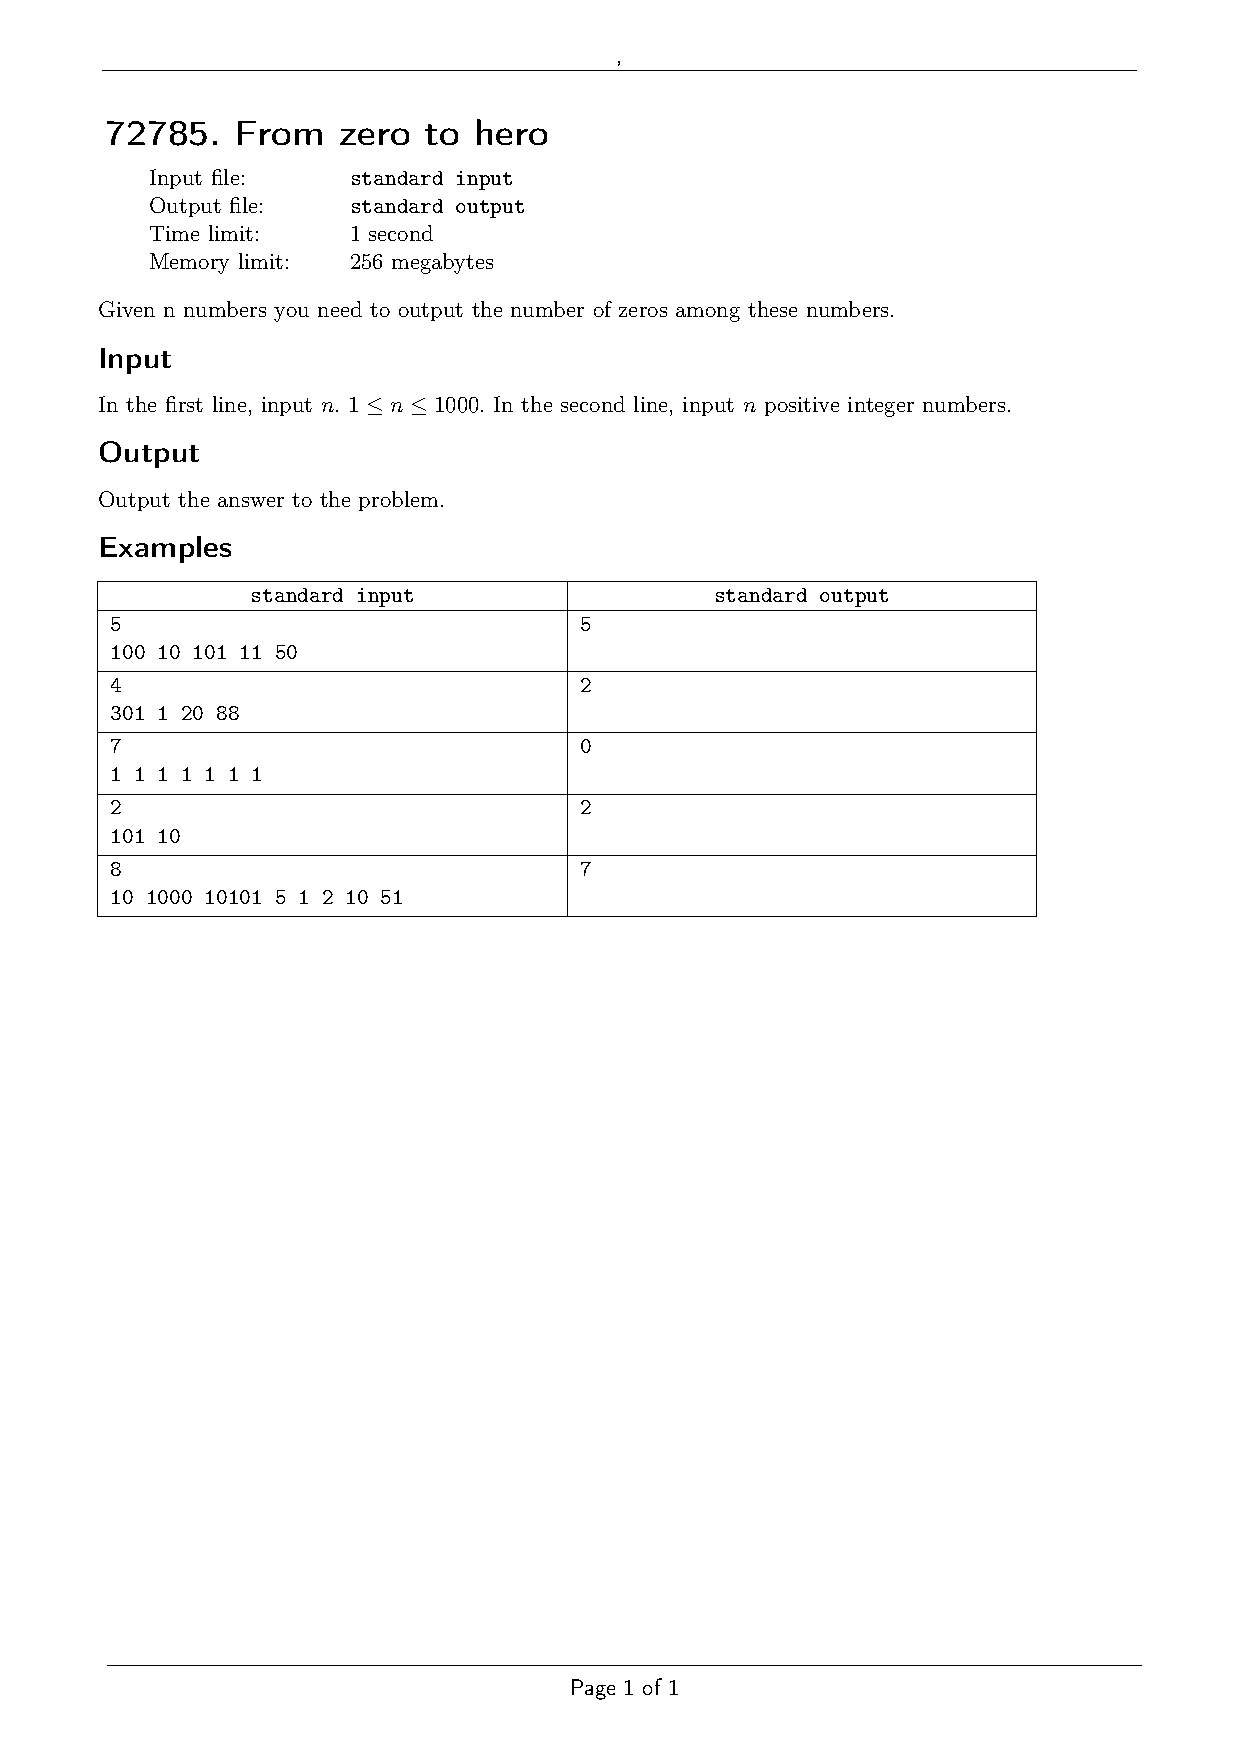
\includepdf[pages=-]{72785.pdf}
    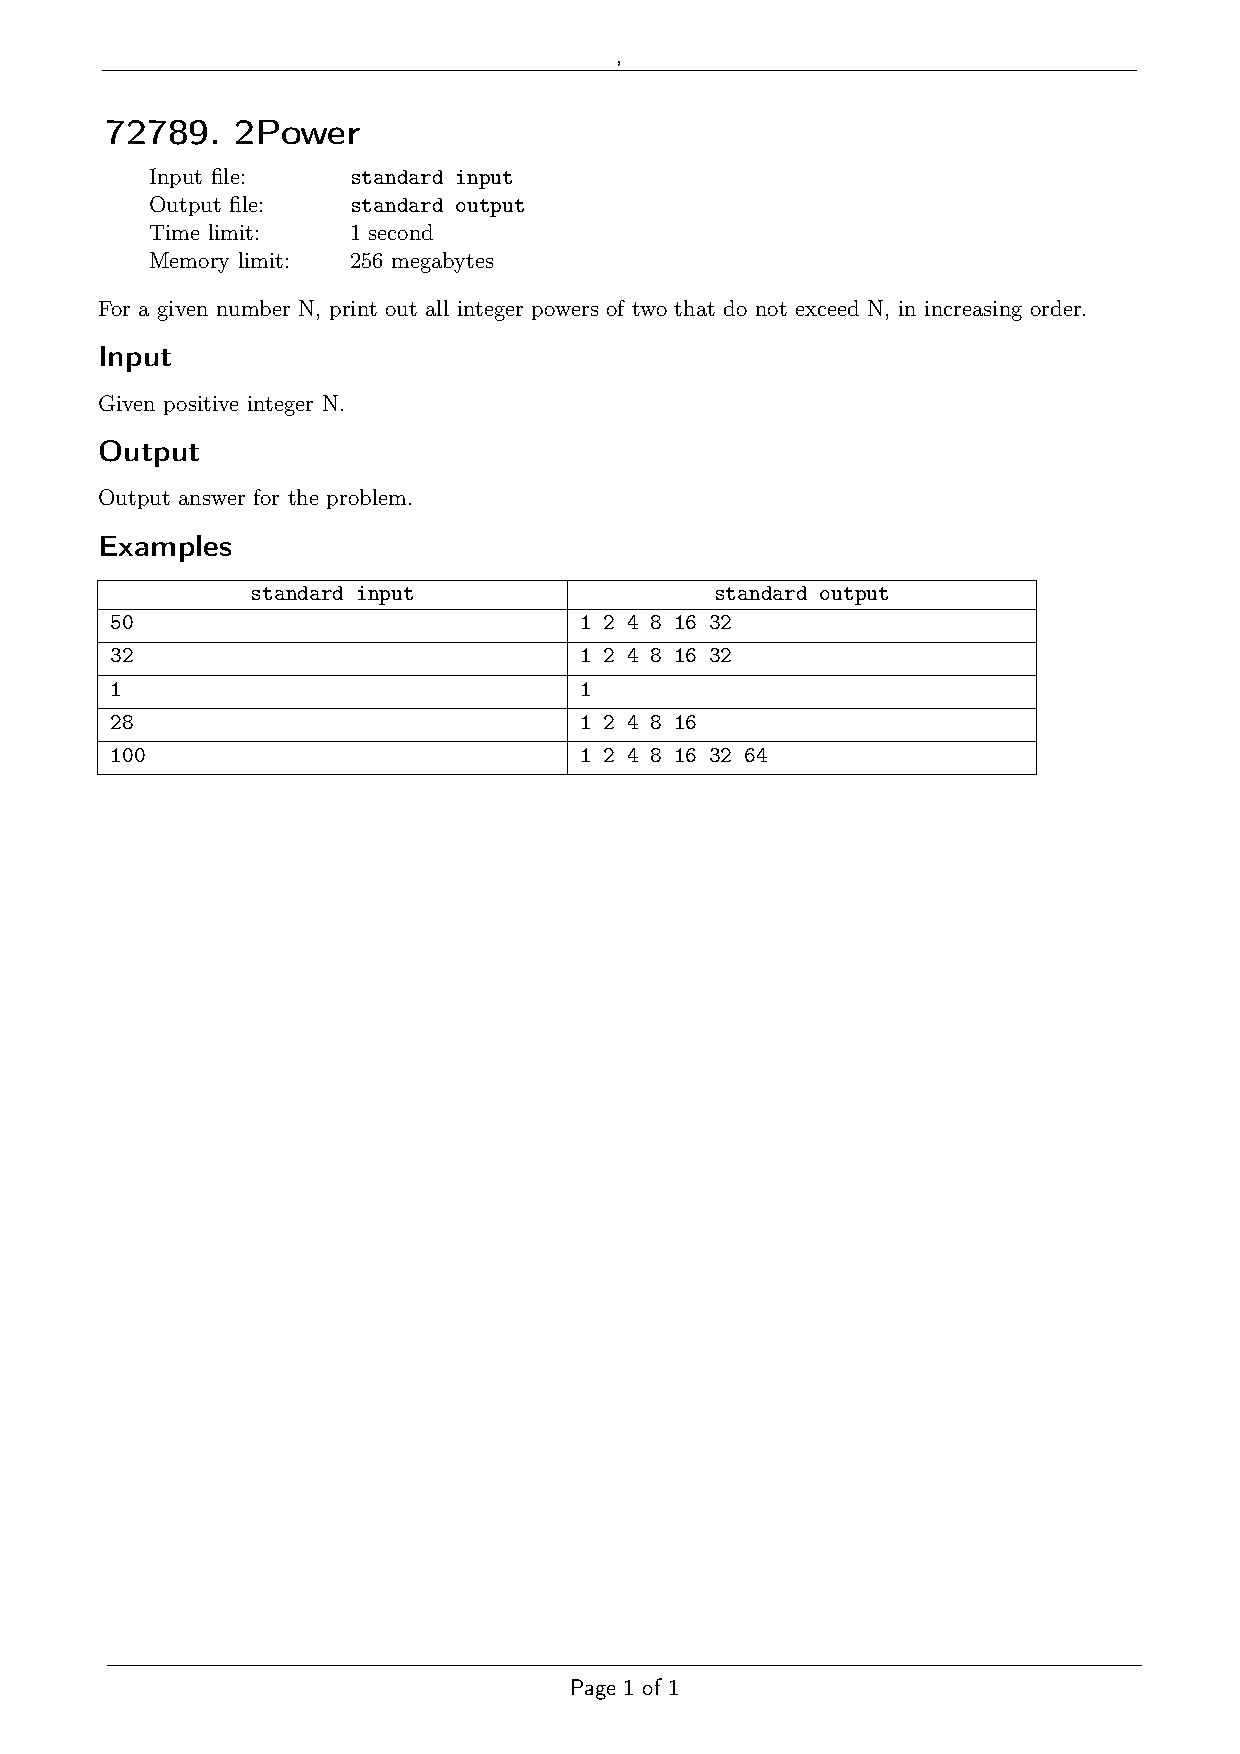
\includepdf[pages=-]{72789.pdf}
    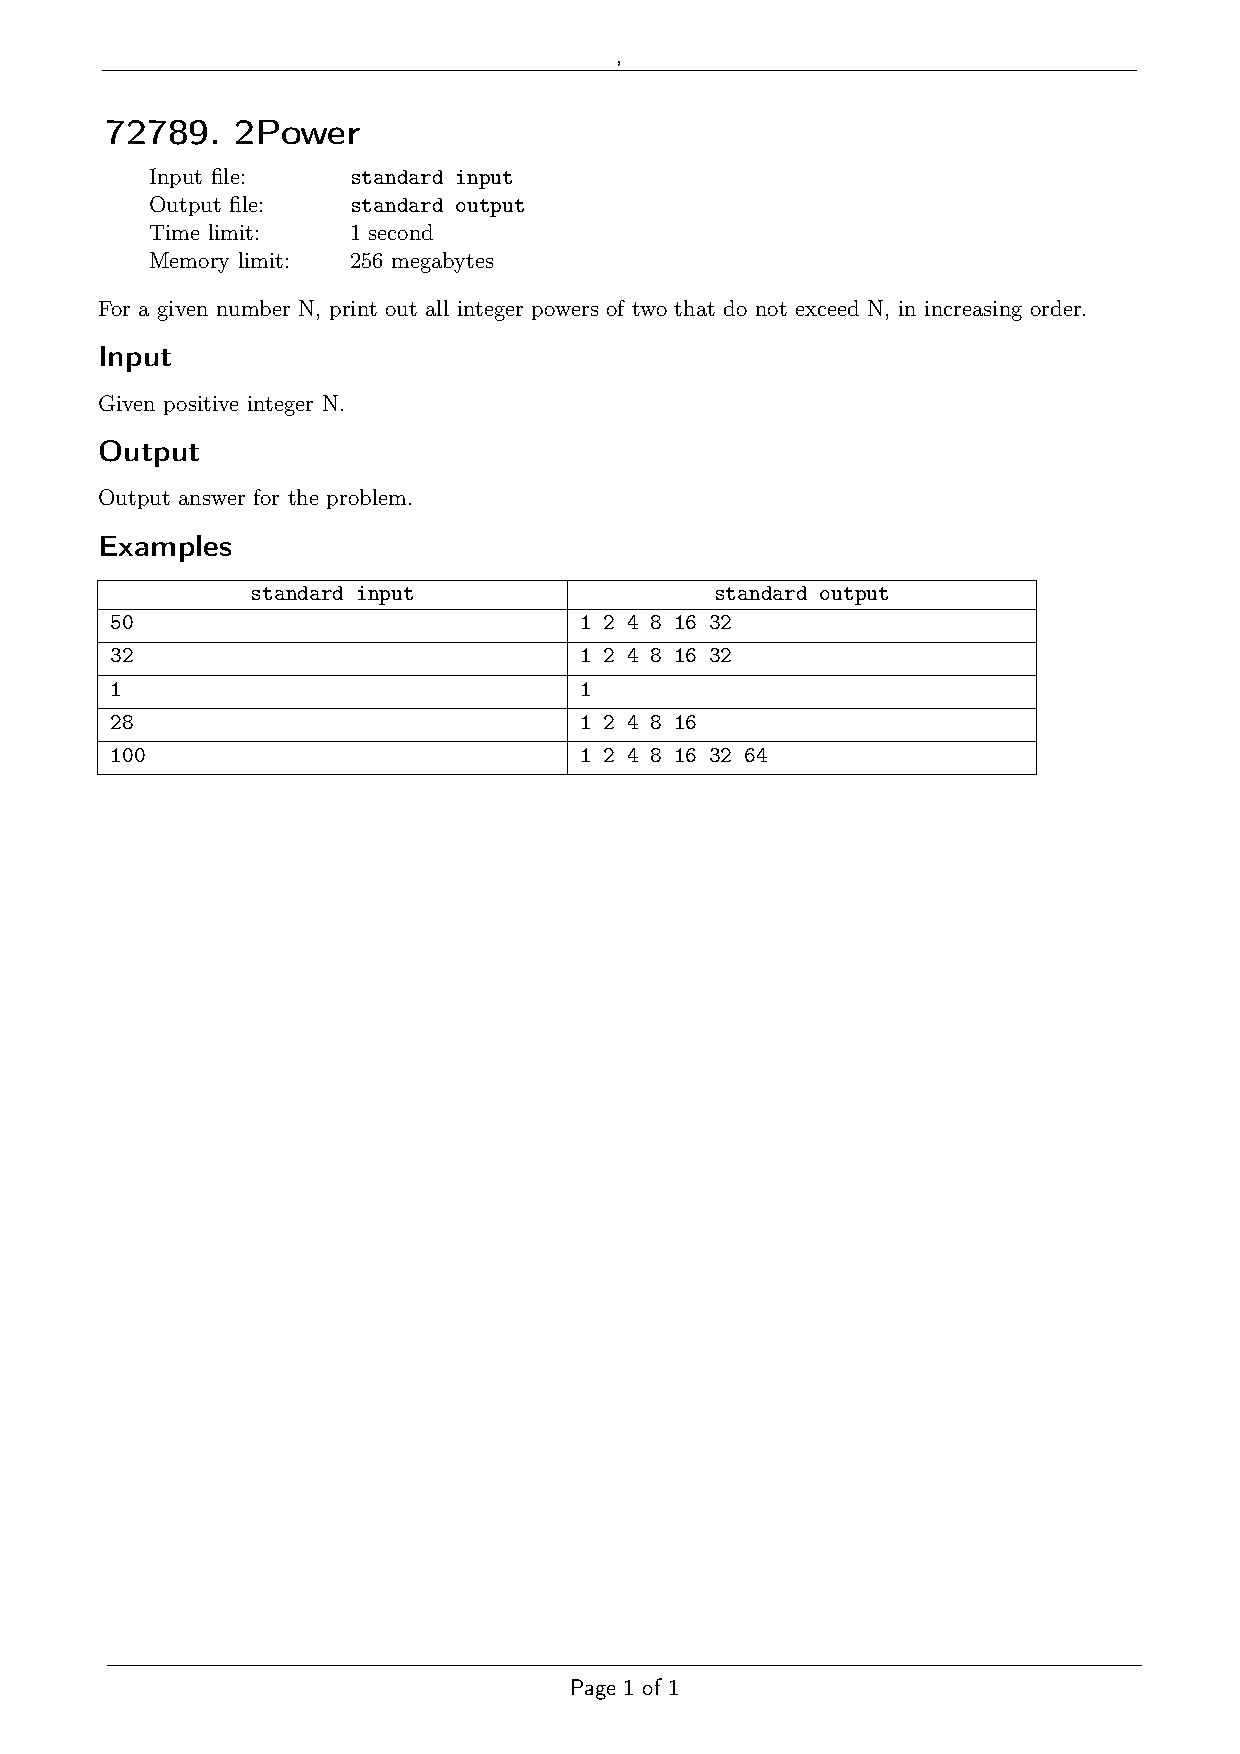
\includepdf[pages=-]{72789.pdf}
    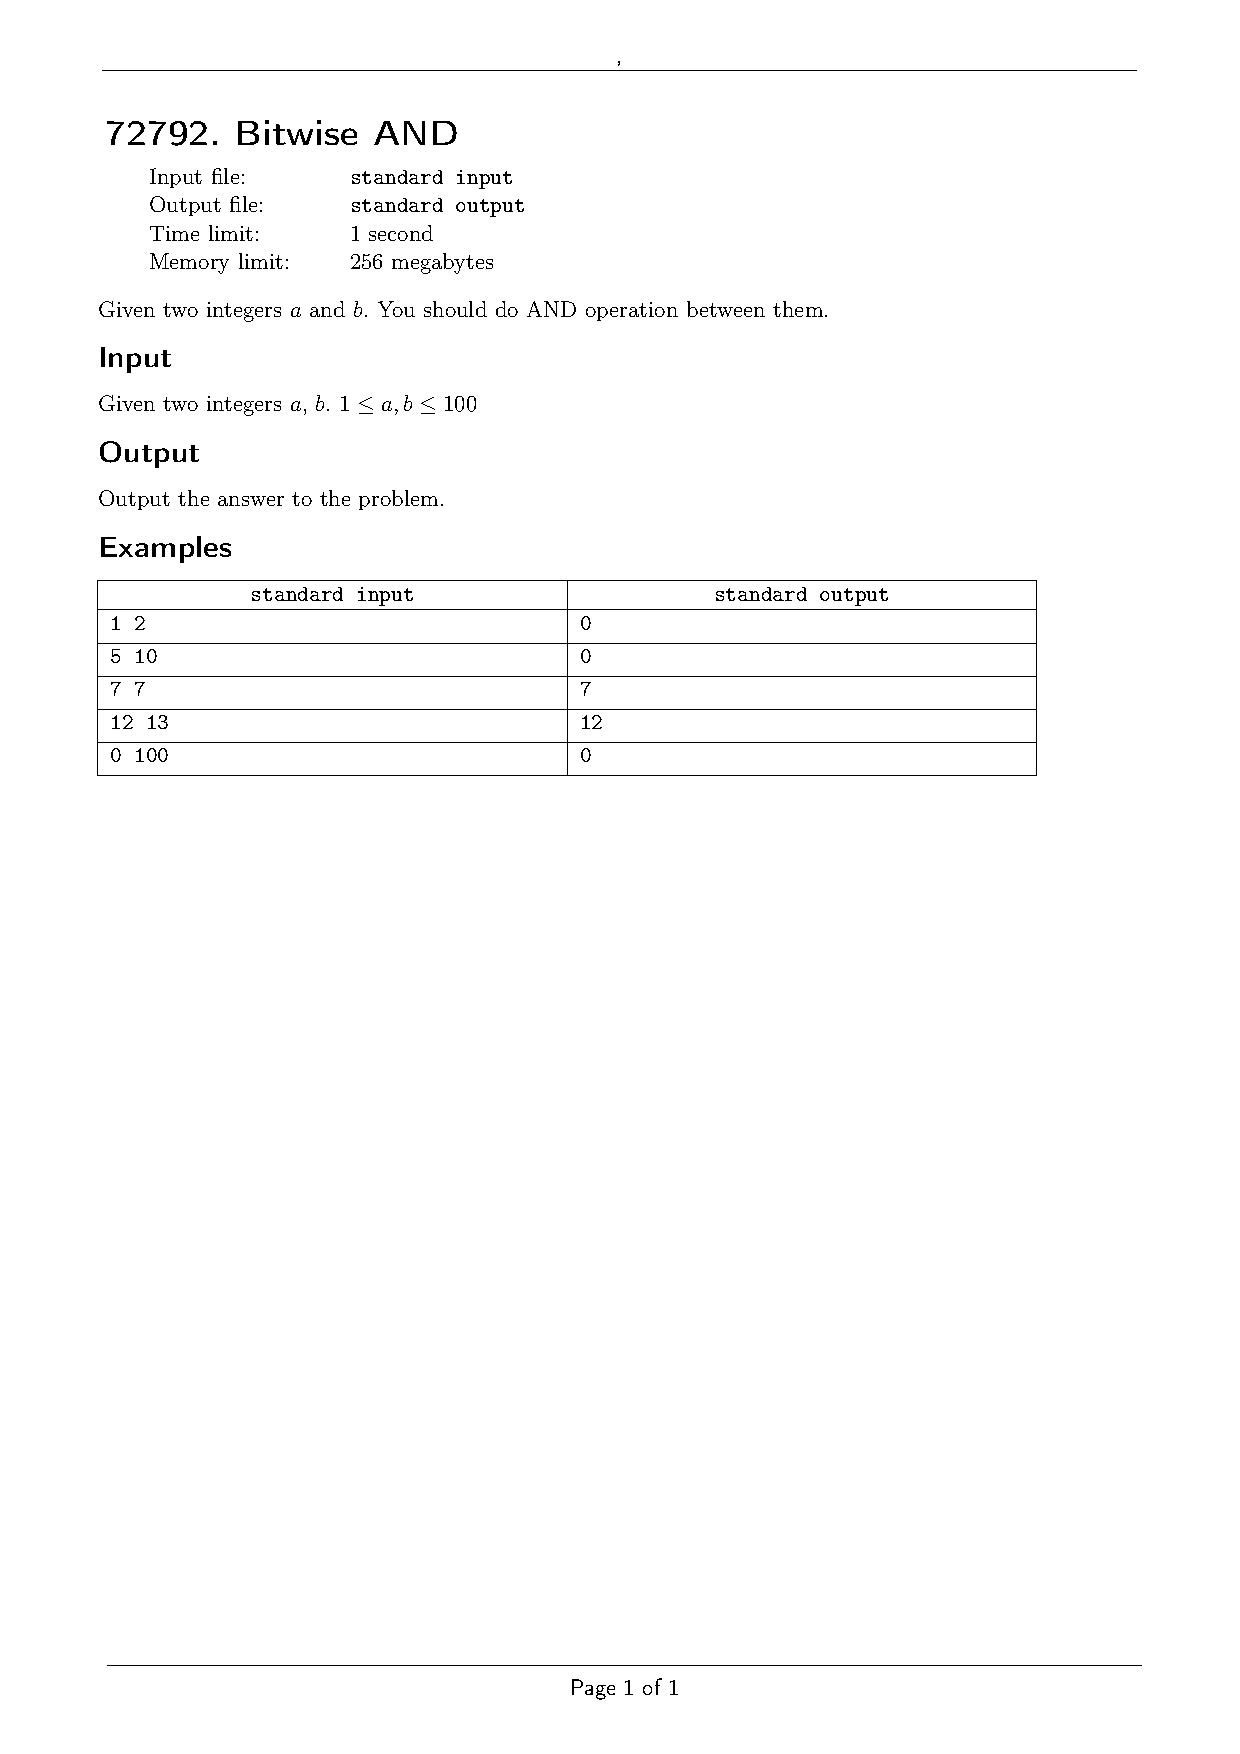
\includepdf[pages=-]{72792.pdf}
    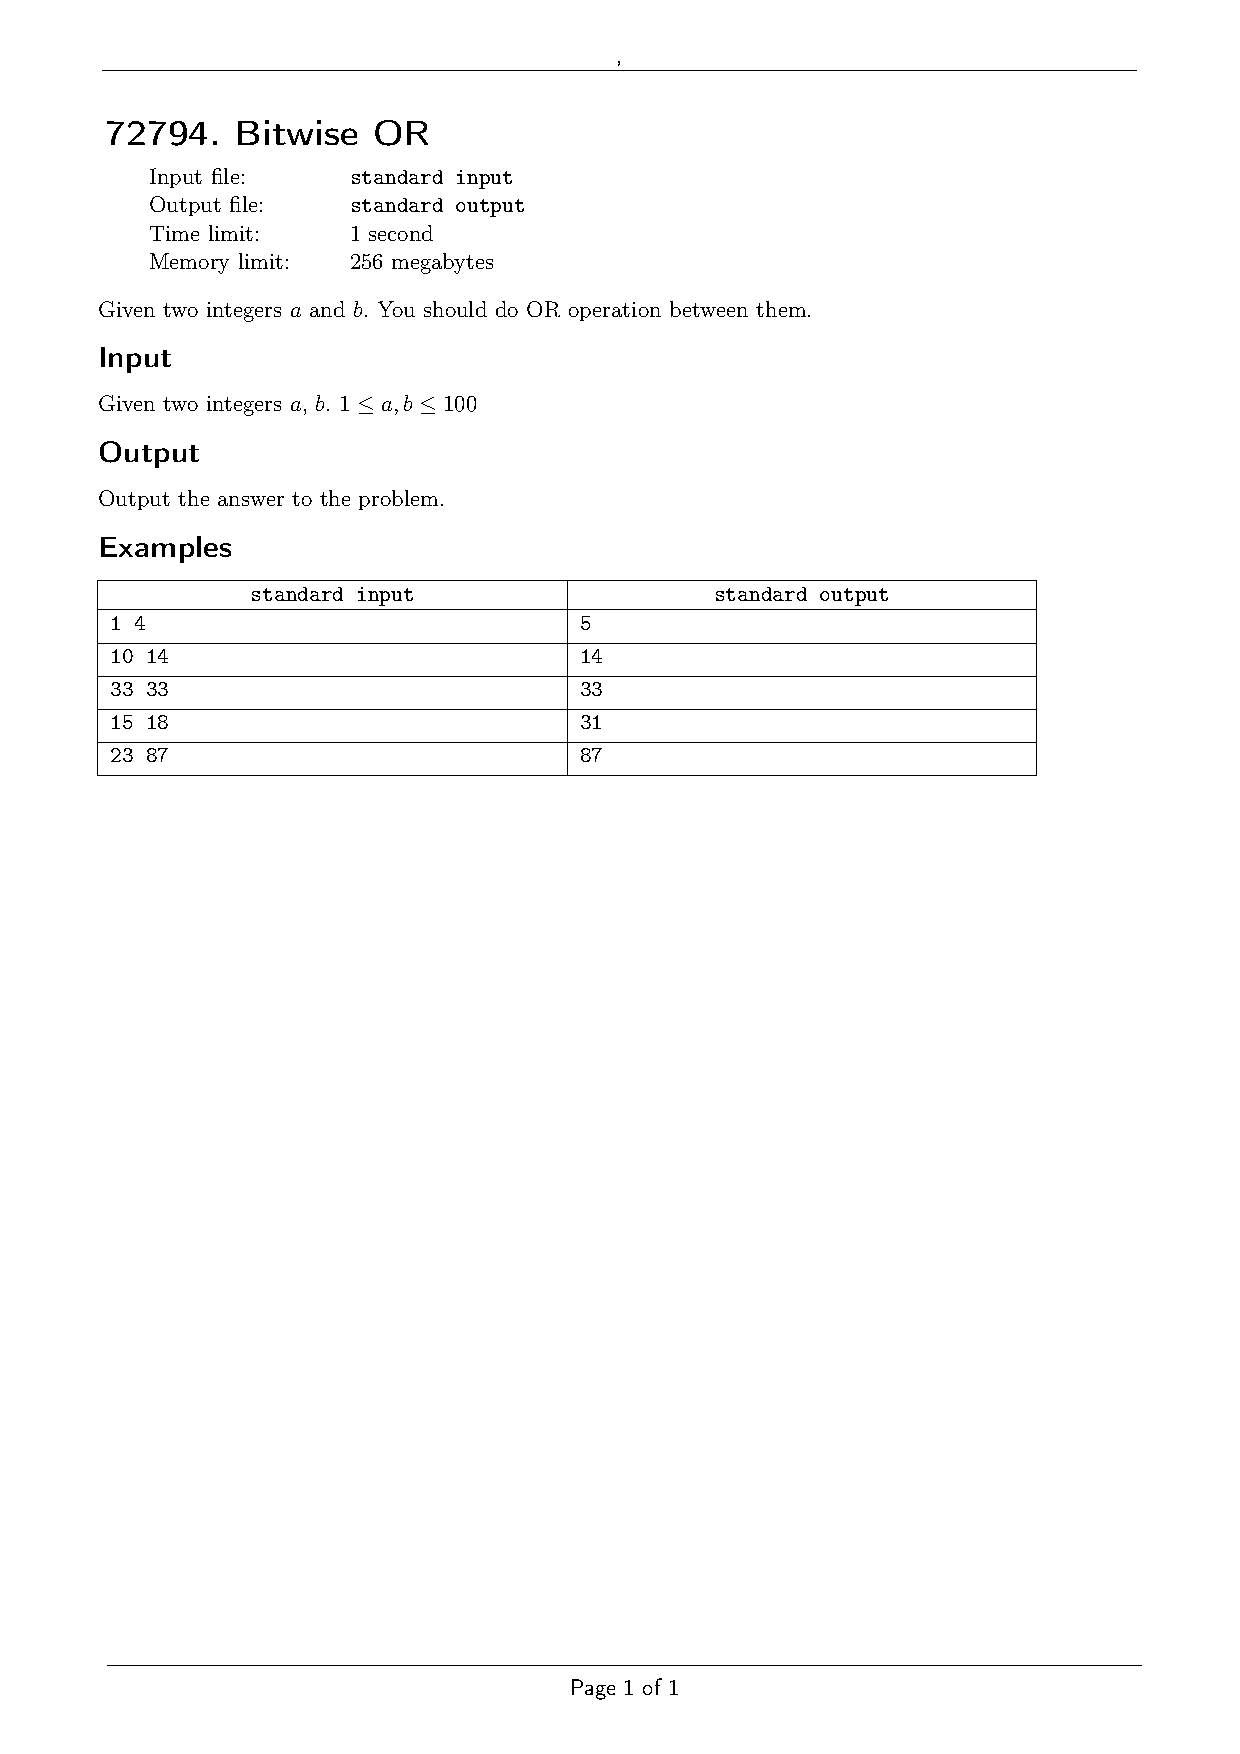
\includepdf[pages=-]{72794.pdf}
    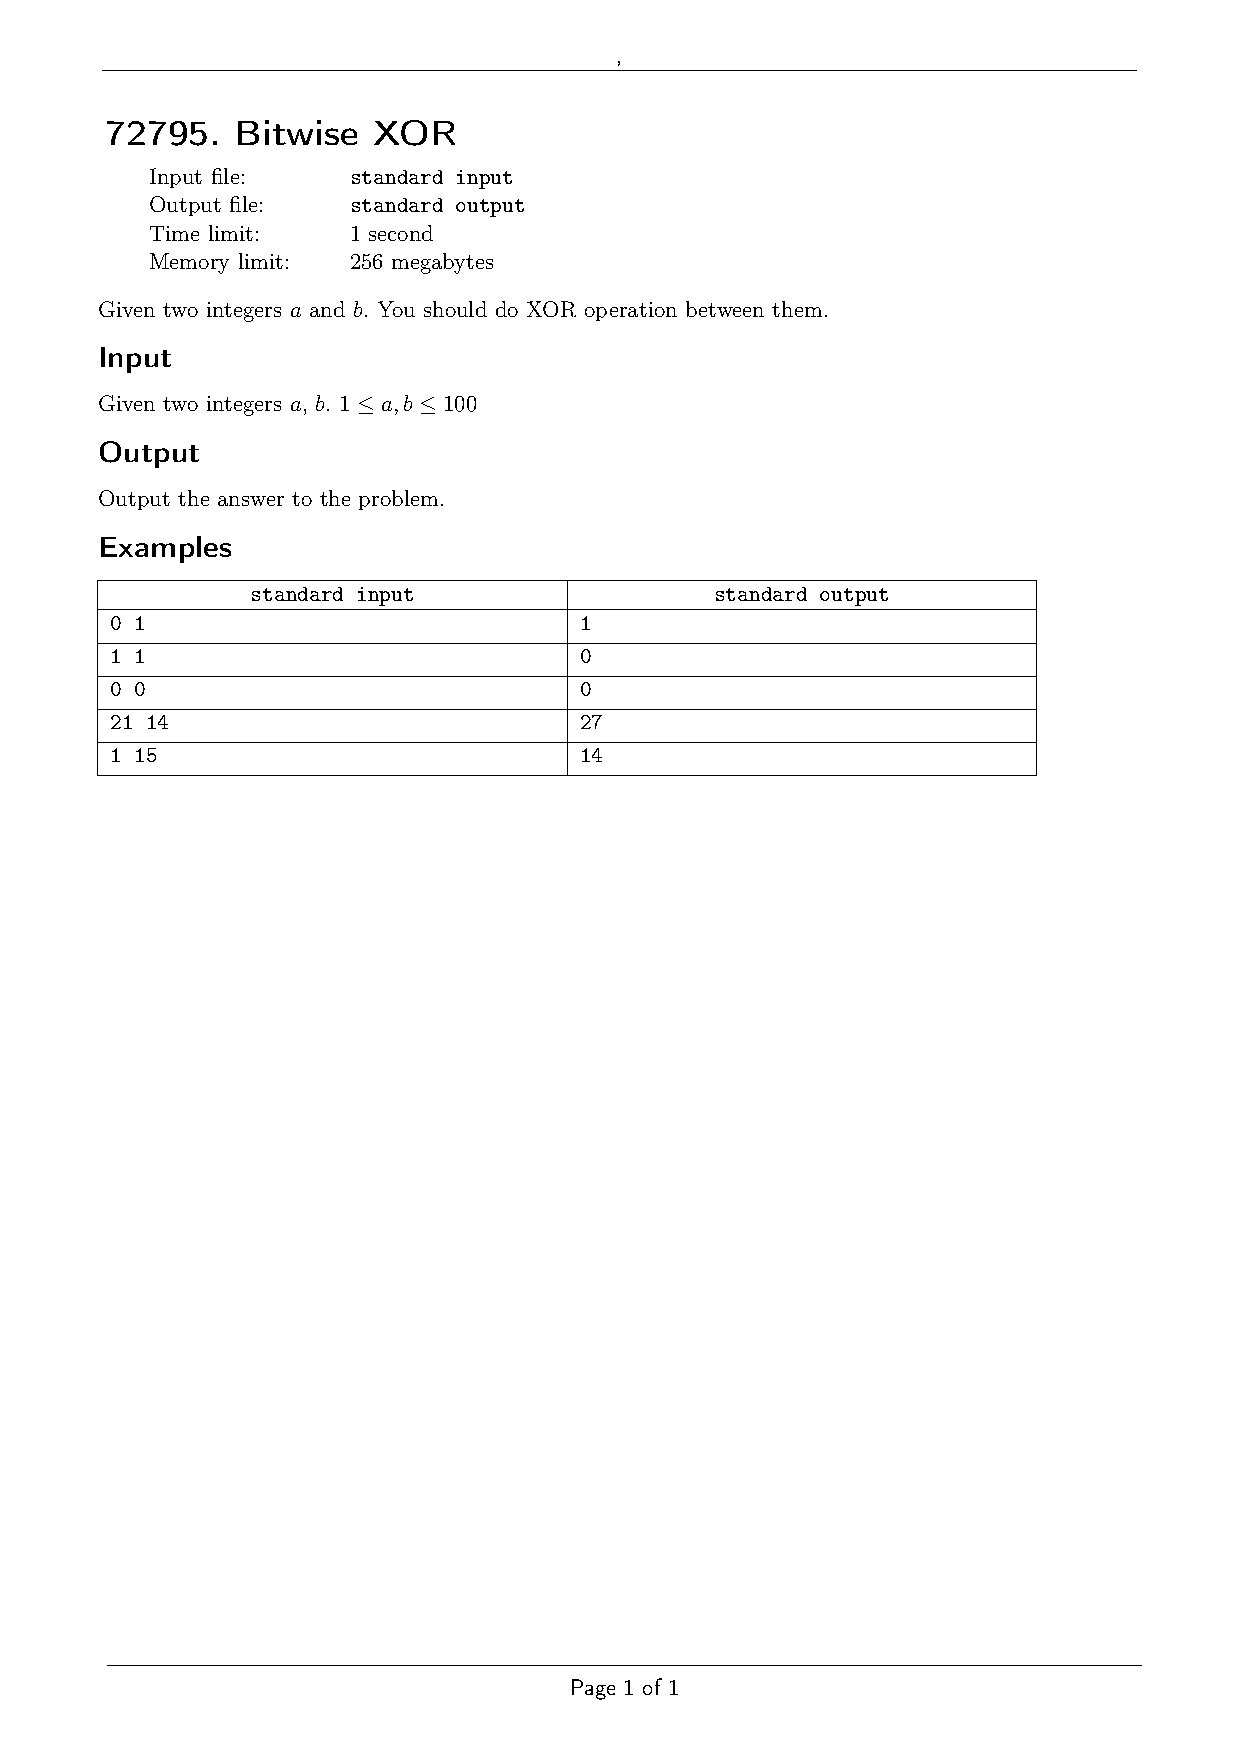
\includepdf[pages=-]{72795.pdf}

    \section{lab contest}
    
    All given tasks are emplaced in automated checker system for \textbf{lab2}: \url{http://acm.kbtu.kz/cgi-bin/new-register?action=211&contest_id=126}\\
    Feel free to submit your solutions without attempt count penalty.

    \section{solutions}

    \textbf{problem 72769}
    \lstinputlisting{72769.cpp}
    \textbf{problem 72770}
    \lstinputlisting{72770.cpp}
    \textbf{problem 72772}
    \lstinputlisting{72772.cpp}
    \textbf{problem 72773}
    \lstinputlisting{72773.cpp}
    \textbf{problem 72776}
    \lstinputlisting{72776.cpp}
    \textbf{problem 72778}
    \lstinputlisting{72778.cpp}
    \textbf{problem 72779}
    \lstinputlisting{72779.cpp}
    \textbf{problem 72782}
    \lstinputlisting{72782.cpp}
    \textbf{problem 72784}
    \lstinputlisting{72784.cpp}
    \textbf{problem 72785}
    \lstinputlisting{72785.cpp}
    \textbf{problem 72789}
    \lstinputlisting{72789.cpp}
    \textbf{problem 72789}
    \lstinputlisting{72789.cpp}
    \textbf{problem 72792}
    \lstinputlisting{72792.cpp}
    \textbf{problem 72794}
    \lstinputlisting{72794.cpp}
    \textbf{problem 72795}
    \lstinputlisting{72795.cpp}

    \section{additional tasks for this lab}
    You can solve some problems from the links below:
    \begin{itemize}
        \item \url{https://informatics.msk.ru/mod/statements/view.php?id=276}
        \item \url{https://informatics.msk.ru/mod/statements/view.php?id=278}
        \item \url{https://informatics.msk.ru/mod/statements/view.php?id=280}
        \item \url{https://informatics.msk.ru/mod/statements/view.php?id=249}
        \item \url{https://informatics.msk.ru/mod/statements/view.php?id=2585}
        \item \url{https://informatics.msk.ru/mod/statements/view.php?id=2587}
    \end{itemize}
    \vspace{5cm}
    \begin{center}
    {\large \emph{Good Luck!}}
    \end{center}
\end{document}